\documentclass[tikz,border=10pt]{standalone}
% Coordinates: x = px/100, y = (922 - py)/100 (y axis flipped from image)
\begin{document}
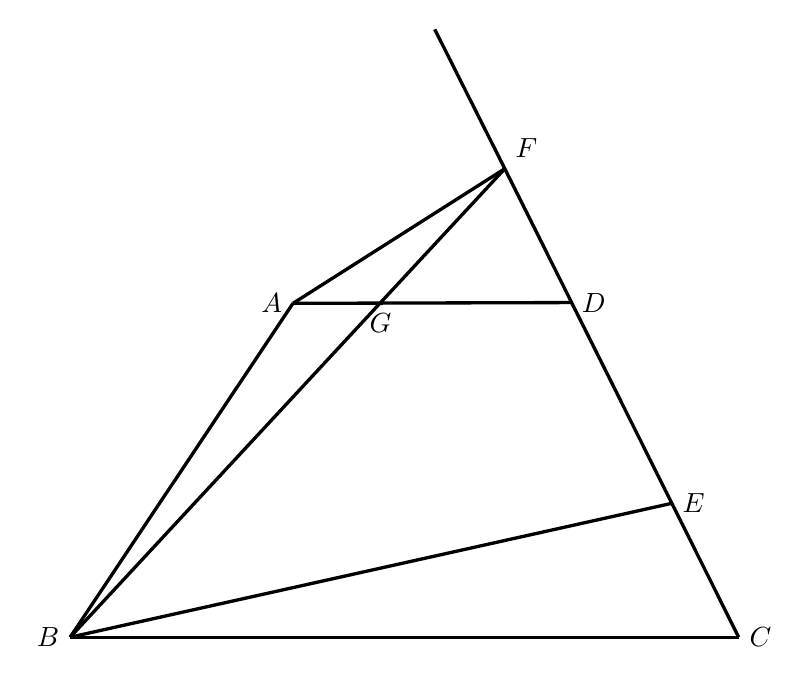
\begin{tikzpicture}[line width=1.2pt, line join=round]
  % Named points
  \coordinate (A) at (4.05,5.13);
  \coordinate (B) at (1.22,0.89);
  \coordinate (C) at (9.71,0.89);
  \coordinate (D) at (7.58,5.14);
  \coordinate (E) at (8.86,2.59);
  \coordinate (F) at (6.74,6.84);
  \coordinate (G) at (5.16,5.14);
  % Free endpoint beyond F on the line C-E-D-F (image px 585,61)
  \coordinate (H) at (5.85,8.61);

  % Baseline
  \draw (B) -- (C);
  % Line C-E-D-F extended past F to H
  \draw (C) -- (F) -- (H);

  % Triangle and auxiliary segments
  \draw (F) -- (B);
  \draw (B) -- (E);
  \draw (B) -- (A);
  \draw (A) -- (F);

  % Horizontal segment A-D (G lies on it)
  \draw (A) -- (D);

  % Vertex labels outside the figure
  \node[left]  at (A) {$A$};
  \node[left]  at (B) {$B$};
  \node[right] at (C) {$C$};
  \node[right] at (D) {$D$};
  \node[right] at (E) {$E$};
  \node[above right] at (F) {$F$};
  \node[below] at (G) {$G$};
\end{tikzpicture}
\end{document}